\documentclass[10pt,a4paper]{article}
\usepackage[margin=17mm,top=15mm,bottom=18mm]{geometry}
\usepackage{fontspec,unicode-math,amsmath,enumitem,xcolor,fancyhdr,lastpage,needspace,tcolorbox,tikz}
\IfFontExistsTF{Arial Unicode MS}{\setmainfont{Arial Unicode MS}\setsansfont{Arial Unicode MS}}{\setmainfont{Noto Sans CJK KR}[BoldFont={Noto Sans CJK KR Bold}]\setsansfont{Noto Sans CJK KR}[BoldFont={Noto Sans CJK KR Bold}]}
\IfFontExistsTF{TeX Gyre Termes Math}{\setmathfont{TeX Gyre Termes Math}}{\setmathfont[Path=/usr/local/texlive/2019/texmf-dist/fonts/opentype/public/tex-gyre-math/]{texgyretermes-math.otf}}
\setlength{\parindent}{0pt}
\setlength{\parskip}{3pt}
\setlength{\emergencystretch}{2em}
\setlist[enumerate]{leftmargin=7mm,itemsep=1pt,topsep=2pt}
\definecolor{navy}{HTML}{0B1F3A}
\definecolor{blue}{HTML}{2563EB}
\definecolor{light}{HTML}{E0F0FE}
\definecolor{hair}{HTML}{D0D5DD}
\definecolor{gray}{HTML}{667085}
\definecolor{ink}{HTML}{191919}
\definecolor{red}{HTML}{B42318}
\pagestyle{fancy}
\fancyhf{}
\lfoot{전자기학 2026 · WEEK 09}
\rfoot{\thepage/\pageref{LastPage}}
\renewcommand{\headrulewidth}{0pt}
\newcommand{\vect}[1]{\symbf{#1}}
\newcommand{\unit}[1]{\hat{\symbf{#1}}}
\newcommand{\dd}{\mathop{}\!\mathrm{d}}
\newcommand{\sepR}{\symscr{r}}
\newcommand{\problem}[3]{%
  \needspace{0.18\textheight}
  \par\vspace{2.2mm}
  {\large\bfseries\color{navy}#1\hfill{\normalsize\color{blue}#2점}}\par
  \smallskip #3\par
}
\newcommand{\sectionbar}[1]{%
  \needspace{0.25\textheight}
  \par\vspace{2.5mm}
  \colorbox{navy}{\parbox{0.965\linewidth}{\color{white}\bfseries\large #1}}
  \par\vspace{0.5mm}
}
\newtcolorbox{infobox}{colback=light,colframe=blue,boxrule=0.5pt,arc=0pt,left=3mm,right=3mm,top=2mm,bottom=2mm}
\newcommand{\answer}[1]{\par\begin{tcolorbox}[colback=white,colframe=hair,boxrule=0.5pt,arc=0pt,left=3mm,right=3mm,top=1.5mm,bottom=1.5mm]{\color{blue}\bfseries 풀이}\quad #1\end{tcolorbox}}
% TikZ 공통 스타일
\tikzset{
  ax/.style={-latex, draw=gray, line width=0.6pt},
  pc/.style={circle, fill=blue, inner sep=0pt, minimum size=4.2pt},
  nc/.style={circle, fill=ink, inner sep=0pt, minimum size=4.2pt},
  lab/.style={font=\small},
}

\begin{document}
\begin{center}
  {\LARGE\bfseries\color{navy}9주차 연습문제 세트 — 풀이}\\[1.5mm]
  {\large 다중극 전개}\\[1mm]
  {\small Griffiths 4판 §3.4 (Problems 3.27--3.36 재구성) · 10월 26일(월)·11월 2일(월) 연습}
\end{center}
\begin{infobox}
\textbf{풀이 원칙}\quad 원점을 먼저 정하고 총전하 $Q$, 쌍극자 모멘트 $\vect p$를 차례로 계산하여 0이 아닌 가장 낮은 차수의 항을 찾으시오. 근사 전위와 전기장은 구 좌표계 $(r,\theta,\phi)$로 쓰고 $1/(4\pi\epsilon_0)$ 인자를 명시하시오. 필요한 식:
\[
\frac{1}{\sepR}=\sum_{n=0}^{\infty}\frac{(r')^n}{r^{n+1}}P_n(\cos\alpha),\qquad
V(\vect r)=\frac{1}{4\pi\epsilon_0}\sum_{n=0}^{\infty}\frac{1}{r^{n+1}}\int (r')^nP_n(\cos\alpha)\,\rho(\vect r')\dd\tau',
\]
\[
\vect p=\int \vect r'\rho(\vect r')\dd\tau',\qquad
P_0=1,\quad P_1(x)=x,\quad P_2(x)=\tfrac12(3x^2-1),\quad P_3(x)=\tfrac12(5x^3-3x).
\]
여기서 $\alpha$는 장점 방향 $\unit r$과 원천점 방향 $\unit r'$ 사이의 각이다.
\end{infobox}

\sectionbar{A. 먼 거리 근사와 르장드르 전개 (§3.4.1) · 34점}
\problem{P1. 비균일 구 분포의 축 위 전위 (Prob.~3.27)}{12}{%

반지름 $R$, 중심이 원점인 구 안($r\le R$)에 전하밀도
\[
\rho(r,\theta)=k\,\frac{R}{r^2}\,(R-2r)\sin\theta
\]
가 분포한다. $k$는 상수이고 구 밖에는 전하가 없다.
\begin{enumerate}[label=(\alph*)]
  \item 총전하 $Q=\int\rho\,\dd\tau$를 구하시오.
  \item $z$축 위의 먼 점($|z|\gg R$)에서는 $\alpha=\theta'$이다. 다중극 전개의 $n=1$ 항이 0임을 보이시오.
  \item 0이 아닌 가장 낮은 차수의 항을 계산하여 $z$축 위 먼 곳의 근사 전위를 구하시오.
\end{enumerate}
\answer{(a) $\dd\tau=r^2\sin\theta\,\dd r\,\dd\theta\,\dd\phi$이므로 $\rho\,\dd\tau=kR(R-2r)\sin^2\theta\,\dd r\,\dd\theta\,\dd\phi$.
$\int_0^R(R-2r)\dd r=R^2-R^2=0$이므로 $Q=0$.

(b) $n=1$ 항의 적분 $=2\pi kR\int_0^R r(R-2r)\dd r\int_0^\pi\sin^2\theta\cos\theta\,\dd\theta$. 각 적분 $=[\sin^3\theta/3]_0^\pi=0$이므로 0. (지름 적분 $-R^3/6$은 0이 아니지만 각 적분이 0.)

(c) $n=2$: 지름 적분 $\int_0^R r^2(R-2r)\dd r=R^4/3-R^4/2=-R^4/6$,
각 적분 $\int_0^\pi\sin^2\theta\,P_2(\cos\theta)\dd\theta=\tfrac12\big(3\cdot\tfrac{\pi}{8}-\tfrac{\pi}{2}\big)=-\tfrac{\pi}{16}$.
\[
\int (r')^2P_2\rho\,\dd\tau'=2\pi kR\Big(-\frac{R^4}{6}\Big)\Big(-\frac{\pi}{16}\Big)=\frac{\pi^2kR^5}{48},
\qquad
\boxed{V(z)\approx\frac{1}{4\pi\epsilon_0}\frac{\pi^2kR^5}{48\,|z|^3}=\frac{\pi kR^5}{192\,\epsilon_0|z|^3}}
\]
$P_2(\pm1)=1$이므로 $z>0$, $z<0$ 모두 같은 식이다. 4중극자 항이 주도한다.}}
\problem{P2. 균일하게 대전된 원형 고리 (Prob.~3.28)}{12}{%

$xy$ 평면에 반지름 $R$, 중심이 원점인 원형 고리가 있고 균일한 선전하밀도 $\lambda$를 갖는다.
\begin{enumerate}[label=(\alph*)]
  \item 고리 위의 원천점 $\vect r'=(R,\pi/2,\phi')$과 장점 $\vect r=(r,\theta,\phi)$ 사이의 각 $\alpha$에 대해 $\cos\alpha=\sin\theta\cos(\phi-\phi')$임을 보이시오.
  \item 다중극 전개의 처음 세 항($n=0,1,2$)을 구하여 $V(r,\theta)$를 근사하시오.
  \item $z$축 위의 정확한 전위 $V(z)=\dfrac{1}{4\pi\epsilon_0}\dfrac{2\pi R\lambda}{\sqrt{z^2+R^2}}$를 $R/z$로 전개하여 (b)와 비교하시오.
\end{enumerate}
\answer{(a) $\unit r=(\sin\theta\cos\phi,\sin\theta\sin\phi,\cos\theta)$, $\unit r'=(\cos\phi',\sin\phi',0)$이므로 $\cos\alpha=\unit r\cdot\unit r'=\sin\theta\cos(\phi-\phi')$.

(b) $\dd q=\lambda R\,\dd\phi'$.
$n=0$: $\dfrac{1}{4\pi\epsilon_0}\dfrac{2\pi R\lambda}{r}$. \quad
$n=1$: $\int\cos(\phi-\phi')\dd\phi'=0$이므로 0.\quad
$n=2$: $\int_0^{2\pi}P_2(\cos\alpha)\dd\phi'=\tfrac{3\pi}{2}\sin^2\theta-\pi=-\pi P_2(\cos\theta)$.
\[
\boxed{V(r,\theta)\approx\frac{1}{4\pi\epsilon_0}\frac{2\pi R\lambda}{r}\Big[1-\frac{R^2}{2r^2}P_2(\cos\theta)\Big]}
\]
(c) $\dfrac{1}{\sqrt{z^2+R^2}}=\dfrac1z\Big(1-\dfrac{R^2}{2z^2}+\cdots\Big)$. $\theta=0$에서 $P_2=1$이므로 (b)와 일치한다.}}
\problem{P3. 물리적 쌍극자의 고차항 (Prob.~3.31)}{10}{%

점전하 $+q$가 $(0,0,d/2)$에, $-q$가 $(0,0,-d/2)$에 있다. 장점까지의 거리를 $r_\pm$라 한다.
\begin{enumerate}[label=(\alph*)]
  \item $1/r_\pm$를 $(d/r)^3$ 차수까지 전개하시오.
  \item 4중극자 항이 사라지는 이유를 전하 배치의 대칭으로 설명하시오.
  \item 8중극자 항을 구하여 $P_3(\cos\theta)$로 나타내시오.
\end{enumerate}
\answer{(a) $+q$에 대해 $\alpha=\theta$, $-q$에 대해 $\alpha=\pi-\theta$이므로
\[
\frac{1}{r_\pm}=\frac1r\Big[1\pm\frac{d}{2r}P_1+\Big(\frac{d}{2r}\Big)^2P_2\pm\Big(\frac{d}{2r}\Big)^3P_3+\cdots\Big],\qquad P_n=P_n(\cos\theta).
\]
(b) 짝수 차수 $P_n(-x)=P_n(x)$ 항은 두 전하에서 크기가 같고 부호가 반대여서 상쇄된다. ($z\to-z$ 반사에 대해 배치가 반대칭.)

(c) $V=\dfrac{q}{4\pi\epsilon_0}\Big(\dfrac1{r_+}-\dfrac1{r_-}\Big)$이므로
\[
\boxed{V\approx\frac{1}{4\pi\epsilon_0}\Big[\frac{qd\cos\theta}{r^2}+\frac{qd^3}{4r^4}P_3(\cos\theta)\Big]
=\frac{1}{4\pi\epsilon_0}\frac{qd}{r^2}\Big[\cos\theta+\frac{d^2}{8r^2}(5\cos^3\theta-3\cos\theta)\Big]}
\]}}

\sectionbar{B. 홀극·쌍극자 항과 원점의 선택 (§3.4.2–§3.4.3) · 32점}
\problem{P4. 네 점전하의 먼 거리 전위 (Prob.~3.29)}{10}{%
\begin{minipage}[t]{0.64\linewidth}\vspace{0pt}
원점에서 거리 $a$인 네 점에 점전하가 있다: $3q$는 $(0,0,a)$, $q$는 $(0,0,-a)$, $-2q$는 $(0,a,0)$과 $(0,-a,0)$.
\begin{enumerate}[label=(\alph*)]
  \item 총전하 $Q$를 구하시오.
  \item 쌍극자 모멘트 $\vect p$를 구하시오.
  \item 원점에서 먼 점에서 성립하는 간단한 근사 전위를 구 좌표계로 쓰시오.
\end{enumerate}\end{minipage}\hfill\begin{minipage}[t]{0.33\linewidth}\vspace{0pt}\centering 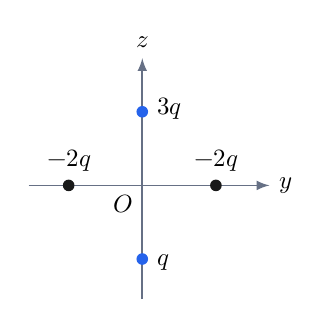
\begin{tikzpicture}[scale=0.85]
\draw[ax] (-1.7,0)--(1.9,0) node[right,lab]{$y$};
\draw[ax] (0,-1.7)--(0,1.9) node[above,lab]{$z$};
\node[pc] at (0,1.1) {}; \node[lab,right] at (0.08,1.15) {$3q$};
\node[pc] at (0,-1.1) {}; \node[lab,right] at (0.08,-1.15) {$q$};
\node[nc] at (-1.1,0) {}; \node[lab,above] at (-1.1,0.06) {$-2q$};
\node[nc] at (1.1,0) {}; \node[lab,above] at (1.1,0.06) {$-2q$};
\node[lab,below left] at (0,0) {$O$};
\end{tikzpicture}\end{minipage}
\answer{(a) $Q=3q+q-2q-2q=0$.\quad
(b) $\vect p=\sum q_i\vect r_i=3qa\unit z-qa\unit z-2qa\unit y+2qa\unit y=2qa\,\unit z$.\quad
(c) $Q=0$이므로 쌍극자 항이 주도한다:
\[\boxed{V(r,\theta)\approx\frac{1}{4\pi\epsilon_0}\frac{2qa\cos\theta}{r^2}}\]}}
\problem{P5. $\cos\theta$ 면전하를 가진 구껍질 (Prob.~3.30)}{10}{%

반지름 $R$인 구껍질에 면전하밀도 $\sigma(\theta)=k\cos\theta$가 분포한다. 예제 3.9에서 구한 이 분포의 정확한 바깥 전위는 다음과 같다.
\[
V(r,\theta)=\frac{kR^3}{3\epsilon_0}\frac{\cos\theta}{r^2}\qquad(r\ge R)
\]
\begin{enumerate}[label=(\alph*)]
  \item 총전하와 쌍극자 모멘트 $\vect p$를 구하시오.
  \item 먼 곳의 쌍극자 근사 전위를 구하여 정확한 전위와 비교하시오.
  \item 비교 결과로부터 이 분포의 고차 다중극 항에 대해 어떤 결론을 내릴 수 있는가?
\end{enumerate}
\answer{(a) $Q=2\pi kR^2\int_0^\pi\cos\theta\sin\theta\,\dd\theta=0$. 대칭으로 $\vect p\parallel\unit z$:
$p_z=\int R\cos\theta\,\sigma\,\dd a=2\pi kR^3\int_0^\pi\cos^2\theta\sin\theta\,\dd\theta=\tfrac{4\pi}{3}kR^3$, \quad $\boxed{\vect p=\tfrac{4\pi}{3}kR^3\,\unit z}$.

(b) $V_{\rm dip}=\dfrac{1}{4\pi\epsilon_0}\dfrac{p\cos\theta}{r^2}=\dfrac{kR^3}{3\epsilon_0}\dfrac{\cos\theta}{r^2}$로, 정확한 전위와 완전히 같다.

(c) 바깥 영역에서 4중극자 이상의 모든 고차 항이 0이다. 구 바깥에서는 순수한 쌍극자 장이다.}}
\problem{P6. 원점의 선택과 쌍극자 모멘트 (Prob.~3.32)}{12}{%

점전하 $3q$와 $-q$가 거리 $a$만큼 떨어져 있다. 다음 세 배치 각각에 대해 (i) 홀극 모멘트, (ii) 쌍극자 모멘트, (iii) 큰 $r$에서 홀극 항과 쌍극자 항을 모두 포함한 근사 전위(구 좌표계)를 구하시오.
\begin{itemize}[leftmargin=7mm,itemsep=0pt]
  \item[(가)] $-q$는 원점, $3q$는 $(0,0,a)$ \quad (나) $3q$는 원점, $-q$는 $(0,0,-a)$ \quad (다) $-q$는 원점, $3q$는 $(0,a,0)$
\end{itemize}
\begin{center}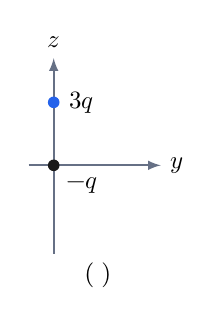
\begin{tikzpicture}[scale=0.8]
\draw[ax] (-0.4,0)--(1.7,0) node[right,lab]{$y$};
\draw[ax] (0,-1.4)--(0,1.7) node[above,lab]{$z$};
\node[nc] at (0,0) {}; \node[lab,below right=1pt] at (0,0) {$-q$};
\node[pc] at (0,1.0) {}; \node[lab,right=2pt] at (0,1.0) {$3q$};
\node[lab] at (0.7,-1.75) {(가)};
\end{tikzpicture}\hspace{8mm}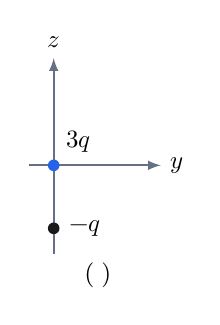
\begin{tikzpicture}[scale=0.8]
\draw[ax] (-0.4,0)--(1.7,0) node[right,lab]{$y$};
\draw[ax] (0,-1.4)--(0,1.7) node[above,lab]{$z$};
\node[pc] at (0,0) {}; \node[lab,above right=1pt] at (0,0) {$3q$};
\node[nc] at (0,-1.0) {}; \node[lab,right=2pt] at (0,-1.0) {$-q$};
\node[lab] at (0.7,-1.75) {(나)};
\end{tikzpicture}\hspace{8mm}\begin{tikzpicture}[scale=0.8]
\draw[ax] (-0.4,0)--(1.7,0) node[right,lab]{$y$};
\draw[ax] (0,-1.4)--(0,1.7) node[above,lab]{$z$};
\node[nc] at (0,0) {}; \node[lab,above left=1pt] at (0,0) {$-q$};
\node[pc] at (1.0,0) {}; \node[lab,above=2pt] at (1.0,0) {$3q$};
\node[lab] at (0.7,-1.75) {(다)};
\end{tikzpicture}\end{center}
(d) (가)와 (나)는 같은 배치를 원점만 달리 잡은 것이다. $\bar{\vect p}=\vect p-Q\vect a$를 이용하여 두 쌍극자 모멘트의 차이를 설명하시오.
\answer{세 배치 모두 $Q=2q$.
\[
\text{(가)}\ \vect p=3qa\,\unit z,\quad V\approx\frac{1}{4\pi\epsilon_0}\Big(\frac{2q}{r}+\frac{3qa\cos\theta}{r^2}\Big);\qquad
\text{(나)}\ \vect p=qa\,\unit z,\quad V\approx\frac{1}{4\pi\epsilon_0}\Big(\frac{2q}{r}+\frac{qa\cos\theta}{r^2}\Big);
\]
\[
\text{(다)}\ \vect p=3qa\,\unit y,\quad V\approx\frac{1}{4\pi\epsilon_0}\Big(\frac{2q}{r}+\frac{3qa\sin\theta\sin\phi}{r^2}\Big).
\]
(d) (나)의 원점은 (가)의 원점을 $\vect a=a\unit z$만큼 옮긴 것($3q$의 위치)이다. $\bar{\vect p}=3qa\unit z-2q\,a\unit z=qa\unit z$. $Q\ne0$이므로 쌍극자 모멘트가 원점에 의존한다.}}

\sectionbar{C. 쌍극자의 전기장과 먼 거리 장 (§3.4.4) · 34점}
\problem{P7. 순수 쌍극자가 점전하에 주는 힘과 일 (Prob.~3.33)}{9}{%

순수(점) 쌍극자 $\vect p=p\,\unit z$가 원점에 있다.
\begin{enumerate}[label=(\alph*)]
  \item 점 $(a,0,0)$에 놓인 점전하 $q$가 받는 힘을 구하시오.
  \item 점 $(0,0,a)$에 놓인 $q$가 받는 힘을 구하시오.
  \item $q$를 $(a,0,0)$에서 $(0,0,a)$로 옮기는 데 필요한 일을 구하고, 이 값이 경로에 무관한 이유를 쓰시오.
\end{enumerate}
\answer{$\vect E_{\rm dip}=\dfrac{p}{4\pi\epsilon_0r^3}(2\cos\theta\,\unit r+\sin\theta\,\unit\theta)$.
(a) $\theta=\pi/2$, $\phi=0$에서 $\unit\theta=-\unit z$: $\boxed{\vect F=-\dfrac{qp}{4\pi\epsilon_0a^3}\unit z}$.\quad
(b) $\theta=0$: $\boxed{\vect F=\dfrac{2qp}{4\pi\epsilon_0a^3}\unit z}$.

(c) $W=q[V(0,0,a)-V(a,0,0)]=q\Big[\dfrac{p}{4\pi\epsilon_0a^2}-0\Big]=\boxed{\dfrac{qp}{4\pi\epsilon_0a^2}}$. 정전기장은 보존장($\nabla\times\vect E=\vect 0$)이므로 경로에 무관하다.}}
\problem{P8. 좌표계에 무관한 쌍극자 장 (Prob.~3.36)}{7}{%

\begin{enumerate}[label=(\alph*)]
  \item $\vect p=p\,\unit z$를 $\unit r$과 $\unit\theta$로 나타내고, 쌍극자 장 $\vect E_{\rm dip}=\dfrac{p}{4\pi\epsilon_0r^3}(2\cos\theta\,\unit r+\sin\theta\,\unit\theta)$가
  \[
  \vect E_{\rm dip}(\vect r)=\frac{1}{4\pi\epsilon_0}\frac{1}{r^3}\big[3(\vect p\cdot\unit r)\unit r-\vect p\big]
  \]
  와 같음을 보이시오.
  \item 이 식으로 P7 (a), (b)의 장을 다시 계산하여 확인하시오.
\end{enumerate}
\answer{(a) $\unit z=\cos\theta\,\unit r-\sin\theta\,\unit\theta$이므로 $\vect p=p\cos\theta\,\unit r-p\sin\theta\,\unit\theta$, $\vect p\cdot\unit r=p\cos\theta$.
$3(\vect p\cdot\unit r)\unit r-\vect p=3p\cos\theta\,\unit r-p\cos\theta\,\unit r+p\sin\theta\,\unit\theta=p(2\cos\theta\,\unit r+\sin\theta\,\unit\theta)$.

(b) $(a,0,0)$: $\vect p\cdot\unit r=0$이므로 $\vect E=-\vect p/(4\pi\epsilon_0a^3)$. \quad $(0,0,a)$: $\unit r=\unit z$이므로 $\vect E=2\vect p/(4\pi\epsilon_0a^3)$. P7과 일치.}}
\problem{P9. 세 점전하의 먼 거리 전기장 (Prob.~3.34)}{9}{%
\begin{minipage}[t]{0.64\linewidth}\vspace{0pt}
원점에서 거리 $a$인 세 점에 점전하가 있다: $q$는 $(0,0,a)$, $-q$는 $(0,a,0)$과 $(0,-a,0)$.
\begin{enumerate}[label=(\alph*)]
  \item 총전하 $Q$와 쌍극자 모멘트 $\vect p$를 구하시오.
  \item 다중극 전개의 가장 낮은 두 차수를 포함한 근사 전위를 구하시오.
  \item 원점에서 먼 점의 근사 전기장 $\vect E(r,\theta)$를 구 좌표계로 구하시오.
\end{enumerate}\end{minipage}\hfill\begin{minipage}[t]{0.33\linewidth}\vspace{0pt}\centering \begin{tikzpicture}[scale=0.85]
\draw[ax] (-1.7,0)--(1.9,0) node[right,lab]{$y$};
\draw[ax] (0,-0.9)--(0,1.9) node[above,lab]{$z$};
\node[pc] at (0,1.1) {}; \node[lab,right] at (0.08,1.15) {$q$};
\node[nc] at (-1.1,0) {}; \node[lab,above] at (-1.1,0.06) {$-q$};
\node[nc] at (1.1,0) {}; \node[lab,above] at (1.1,0.06) {$-q$};
\node[lab,below left] at (0,0) {$O$};
\end{tikzpicture}\end{minipage}
\answer{(a) $Q=q-2q=-q$, \quad $\vect p=qa\unit z-qa\unit y+qa\unit y=qa\,\unit z$.\quad
(b) $V\approx\dfrac{1}{4\pi\epsilon_0}\Big(-\dfrac{q}{r}+\dfrac{qa\cos\theta}{r^2}\Big)$.

(c) $\vect E=-\nabla V$:
\[\boxed{\vect E(r,\theta)\approx\frac{q}{4\pi\epsilon_0}\Big[-\frac{1}{r^2}\unit r+\frac{a}{r^3}\big(2\cos\theta\,\unit r+\sin\theta\,\unit\theta\big)\Big]}\]}}
\problem{P10. 위·아래가 반대로 대전된 속찬 구 (Prob.~3.35)}{9}{%
\begin{minipage}[t]{0.64\linewidth}\vspace{0pt}
반지름 $R$, 중심이 원점인 속찬 구에서 북반구($z>0$)는 균일한 전하밀도 $\rho_0$, 남반구($z<0$)는 $-\rho_0$를 갖는다.
\begin{enumerate}[label=(\alph*)]
  \item 총전하를 구하고, 먼 곳에서 주도하는 다중극 항이 무엇인지 쓰시오.
  \item 쌍극자 모멘트 $\vect p$를 구하시오.
  \item $r\gg R$에서의 근사 전기장 $\vect E(r,\theta)$를 구하시오.
\end{enumerate}\end{minipage}\hfill\begin{minipage}[t]{0.33\linewidth}\vspace{0pt}\centering 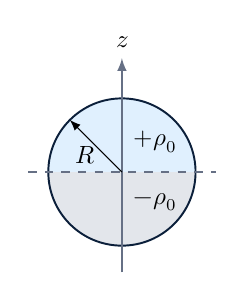
\begin{tikzpicture}[scale=0.85]
\fill[light] (1.1,0) arc (0:180:1.1) -- cycle;
\fill[hair!60] (-1.1,0) arc (180:360:1.1) -- cycle;
\draw[navy, line width=0.7pt] (0,0) circle (1.1);
\draw[gray, dashed] (-1.4,0)--(1.4,0);
\draw[ax] (0,-1.5)--(0,1.7) node[above,lab]{$z$};
\node[lab] at (0.5,0.45) {$+\rho_0$}; \node[lab] at (0.5,-0.45) {$-\rho_0$};
\draw[-latex] (0,0)--(-0.78,0.78); \node[lab] at (-0.55,0.25) {$R$};
\end{tikzpicture}\end{minipage}
\answer{(a) $Q=\rho_0\frac{2\pi R^3}{3}-\rho_0\frac{2\pi R^3}{3}=0$이므로 쌍극자 항이 주도한다.

(b) $p_z=\int z\rho\,\dd\tau=2\rho_0\int_{\rm north}r\cos\theta\,\dd\tau=2\rho_0\cdot2\pi\cdot\frac{R^4}{4}\cdot\frac12=\frac{\pi\rho_0R^4}{2}$, \quad $\boxed{\vect p=\tfrac{\pi}{2}\rho_0R^4\,\unit z}$.

(c) \[\boxed{\vect E(r,\theta)\approx\frac{1}{4\pi\epsilon_0}\frac{\pi\rho_0R^4}{2r^3}(2\cos\theta\,\unit r+\sin\theta\,\unit\theta)=\frac{\rho_0R^4}{8\epsilon_0r^3}(2\cos\theta\,\unit r+\sin\theta\,\unit\theta)}\]}}

\end{document}
